% Appendix A

\chapter{Supporting Results and Reproducibility} % Main appendix title
\label{AppendixA}

\section{Confidence Intervals for the Main Results}

Tables~\ref{tab:main_ci_a} and~\ref{tab:main_ci_b} give every main-table score with its 95\% cluster-bootstrap confidence interval over trials (2000 resamples).

\begin{table}[htbp]
    \centering
    \small
    \caption[Main results with CIs: ROUGE]{ROUGE scores with 95\% trial-level CIs (test set, main protocol).}
    \label{tab:main_ci_a}
    \resizebox{\textwidth}{!}{%
    \begin{tabular}{llll}
        \toprule
        System & ROUGE-1 & ROUGE-2 & ROUGE-L \\
        \midrule
        \tabinput{Tables/main_results_ci_overlap_body.tex}
        \bottomrule
    \end{tabular}}
\end{table}

\begin{table}[htbp]
    \centering
    \small
    \caption[Main results with CIs: BLEU, token F1, BERTScore]{BLEU, token F1 and BERTScore with 95\% trial-level CIs (test set, main protocol). BERTScore is baseline-rescaled.}
    \label{tab:main_ci_b}
    \resizebox{\textwidth}{!}{%
    \begin{tabular}{llll}
        \toprule
        System & BLEU & Token F1 & BERTScore \\
        \midrule
        \tabinput{Tables/main_results_ci_other_body.tex}
        \bottomrule
    \end{tabular}}
\end{table}

\section{Training Dynamics}
\label{sec:training}

Figure~\ref{fig:loss} shows the validation loss (145 examples, 32 trials) after every epoch. It falls monotonically for every run, and early stopping never triggered, so training was budget-limited rather than converged. The three Flan-T5-small seeds trace almost identical curves, with final losses between 1.920 and 1.927. Flan-T5-base with LoRA ends at 2.102 after three epochs, higher than the small model's loss after two epochs, and is still decreasing: within the CPU budget it was under-trained. Validation loss is token-level cross-entropy under teacher forcing and does not reveal decoding pathologies such as the repetition loops of Section~\ref{sec:decoding}, which occurred at the lowest-loss checkpoints.

\begin{figure}[htbp]
    \centering
    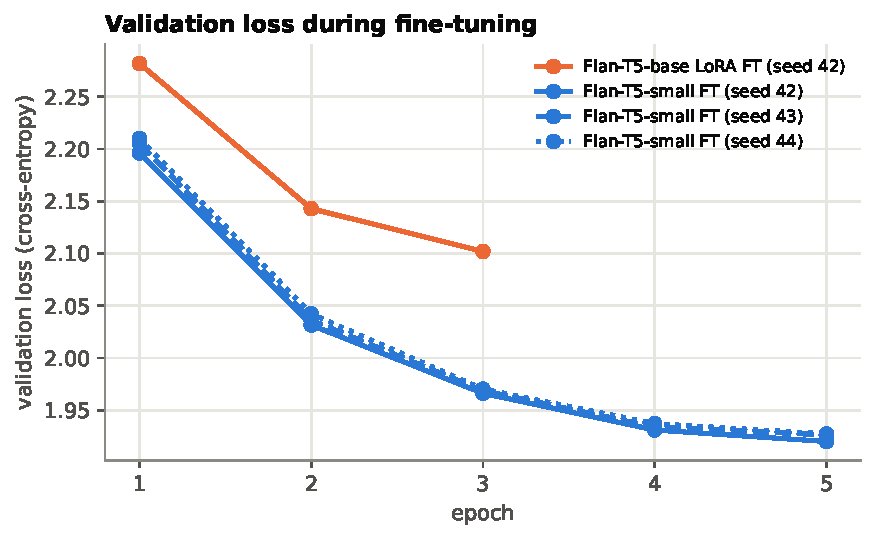
\includegraphics[width=0.85\textwidth]{Figures/results/fig09_validation_loss.pdf}
    \caption[Validation loss]{Validation loss per epoch.}
    \label{fig:loss}
\end{figure}

\section{Compute Cost}
\label{sec:cost}

Table~\ref{tab:cost} gives the median wall-clock generation time per test example (model loading excluded) and the training time. Fine-tuned outputs take longer to generate than zero-shot ones mainly because they are much longer.

\begin{table}[htbp]
    \centering
    \small
    \caption[Compute cost]{Compute cost on the CPU-only machine (8 cores, 15~GB RAM). Latency: median generation time per test example under the main protocol.}
    \label{tab:cost}
    \begin{tabular}{lrrr}
        \toprule
        System & Latency (s) & Training (min) & Epochs \\
        \midrule
        \tabinput{Tables/compute_cost_body.tex}
        \bottomrule
    \end{tabular}
\end{table}

\section{Retrieval Quality of the RAG Index}

The project also contains a retrieval-augmented generation (RAG) layer, which is not part of the summarisation experiments. Its index chunks the report sections of all 212 trials and embeds them with a dependency-free hashing embedder. For each of the 959 (trial, question) pairs, a chunk counts as relevant if it comes from a report section mapped to that question, and retrieval is restricted to the trial. Table~\ref{tab:rag} and Figure~\ref{fig:rag} show that retrieval with this embedder is weak (recall@5 of 0.275, mean reciprocal rank of 0.211), and precision@$k$ stays near 0.10 for every $k$. The relevance labels inherit the question-to-section mapping, so they cover only the seven answerable questions.

\begin{table}[htbp]
    \centering
    \small
    \caption[RAG retrieval]{Retrieval quality of the RAG index (959 queries, retrieval scoped to the trial).}
    \label{tab:rag}
    \begin{tabular}{rrrr}
        \toprule
        $k$ & Recall@$k$ & Precision@$k$ & MRR \\
        \midrule
        \tabinput{Tables/rag_body.tex}
        \bottomrule
    \end{tabular}
\end{table}

\begin{figure}[htbp]
    \centering
    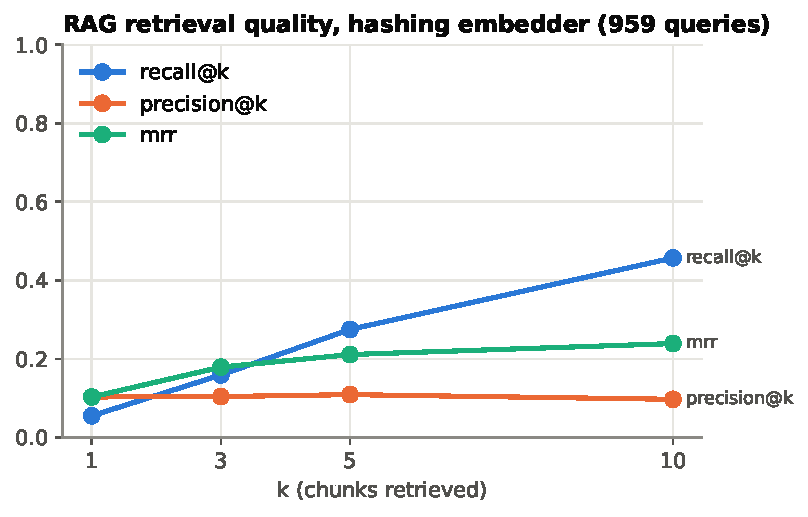
\includegraphics[width=0.7\textwidth]{Figures/results/fig10_rag_retrieval.pdf}
    \caption[RAG retrieval]{Retrieval quality of the RAG index.}
    \label{fig:rag}
\end{figure}

\section{Deviations from the Repository Defaults}
\label{sec:repro}

The experiments use the project's own pipeline, with the changes in Table~\ref{tab:deviations}. The scripts, logs, per-example outputs and notebooks that produced every number are kept with the results.

\begin{table}[htbp]
    \centering
    \small
    \caption[Deviations from repository defaults]{Deviations from the repository defaults applied in all reported runs.}
    \label{tab:deviations}
    \begin{tabularx}{\textwidth}{>{\raggedright\arraybackslash}X>{\raggedright\arraybackslash}X>{\raggedright\arraybackslash}X}
        \toprule
        Repository default & Problem & What this study did \\
        \midrule
        Prompt truncated from the right to 512 tokens, with the question after the context & Long prompts lose the question; training used 1024 tokens & Context capped at 900 Flan-T5 tokens; input limit 1024 tokens \\
        Generation and target limits of 256 tokens & Many test references are longer & 512 tokens \\
        Sampling at temperature 0.7 & Not reproducible & Greedy decoding with no-repeat-3; plain greedy as ablation \\
        Raw prompt for instruction-tuned causal LMs & Ignores the chat format & Chat template applied (Qwen) \\
        No-repeat constraint scans the prompt for decoder-only models & Forbids copying from the source & Constraint applied to generated tokens only \\
        Training batch size 8 & Out of memory & Batch 4 (Flan-T5-small), batch 2 (Flan-T5-base with LoRA) \\
        \bottomrule
    \end{tabularx}
\end{table}
